\documentclass[11pt]{article}
%\usepackage{geometry}
\usepackage[inner=1.5cm,outer=1.5cm,top=2.5cm,bottom=2.5cm]{geometry}
\pagestyle{empty}
\usepackage{graphicx}
\usepackage{fancyhdr, lastpage, bbding, pmboxdraw}
\usepackage[usenames,dvipsnames]{color}
\usepackage{indentfirst}
\definecolor{darkblue}{rgb}{0,0,.6}
\definecolor{darkred}{rgb}{.7,0,0}
\definecolor{darkgreen}{rgb}{0,.6,0}
\definecolor{red}{rgb}{.98,0,0}
\usepackage[colorlinks,pagebackref,pdfusetitle,urlcolor=darkblue,citecolor=darkblue,linkcolor=darkred,bookmarksnumbered,plainpages=false,pdflang=en-US,pdftitle=RadioLab2022]{hyperref}
\renewcommand{\thefootnote}{\fnsymbol{footnote}}

\pagestyle{fancyplain}
\fancyhf{}
\lhead{ \fancyplain{}{AST4723} }
%\chead{ \fancyplain{}{} }
\rhead{ \fancyplain{}{\today} }
%\rfoot{\fancyplain{}{page \thepage\ of \pageref{LastPage}}}
\fancyfoot[RO, LE] {page \thepage\ of \pageref{LastPage} }
\thispagestyle{plain}

%%%%%%%%%%%% LISTING %%%
\usepackage{listings}
\usepackage{caption}
\DeclareCaptionFont{white}{\color{white}}
\DeclareCaptionFormat{listing}{\colorbox{gray}{\parbox{\textwidth}{#1#2#3}}}
\captionsetup[lstlisting]{format=listing,labelfont=white,textfont=white}
\usepackage{verbatim} % used to display code
\usepackage{fancyvrb}
\usepackage{acronym}
\usepackage{amsthm}
\VerbatimFootnotes % Required, otherwise verbatim does not work in footnotes!

\def\todo#1{\textcolor{red}{#1}}


\definecolor{OliveGreen}{cmyk}{0.64,0,0.95,0.40}
\definecolor{CadetBlue}{cmyk}{0.62,0.57,0.23,0}
\definecolor{lightlightgray}{gray}{0.93}



\lstset{
%language=bash,                          % Code langugage
basicstyle=\ttfamily,                   % Code font, Examples: \footnotesize, \ttfamily
keywordstyle=\color{OliveGreen},        % Keywords font ('*' = uppercase)
commentstyle=\color{gray},              % Comments font
numbers=left,                           % Line nums position
numberstyle=\tiny,                      % Line-numbers fonts
stepnumber=1,                           % Step between two line-numbers
numbersep=5pt,                          % How far are line-numbers from code
backgroundcolor=\color{lightlightgray}, % Choose background color
frame=none,                             % A frame around the code
tabsize=2,                              % Default tab size
captionpos=t,                           % Caption-position = bottom
breaklines=true,                        % Automatic line breaking?
breakatwhitespace=false,                % Automatic breaks only at whitespace?
showspaces=false,                       % Dont make spaces visible
showtabs=false,                         % Dont make tabls visible
columns=flexible,                       % Column format
morekeywords={__global__, __device__},  % CUDA specific keywords
}

\begin{document}

\title{Radio Astronomy Lab: HI observations of our Galaxy}
\begin{center}
    {\LARGE  \centering Radio Astronomy Lab: HI observations of our Galaxy}
\end{center}
% 2025 version


In this lab, you will use a small antenna to measure the neutral hydrogen in
our Galaxy.

The lab is set up so that each group will measure a small part of the Galaxy,
then for a final project possibility, we will stitch the different observations
together into one big map.

Your aim in this project is to obtain the data for an assigned part of the sky.
In this lab, you will obtain and calibrate the data.

As a final project, some of you will analyze the data to determine the velocity
of the Galactic neutral hydrogen at two positions.  From this measurement, and
the added information that the sun is 8000 parsecs from the Galactic center,
you will measure the Galaxy's mass.

%Under COVID isolation conditions, each student will work independently.
You will check out the tools described in Section \ref{sec:tools}.

You will do a formal writeup.  The writeup should consist of the following sections:
\begin{enumerate}
    \item Introduction (5\%): Describe the purpose of the lab \& background
    \item Procedure (55\%): Describe the setup of the hardware and the data taking process
    \item Data Analysis (25\%):  Report and analyze your measurements
    \item Data Packaging and Delivery (10\%): Put the data together and turn them in with appropriate metadata
    \item Conclusions (5\%): Summarize what you learned
\end{enumerate}

Upon completing the lab, you can zip up the contents of your folder and send it
to your preferred storage location (e.g., dropbox or google drive).
You may need to log in to the appropriate account on the assigned computer to transfer your data.

\section{Setup and Tools}
\label{sec:tools}

\subsection{Plan your observations}
The \textbf{Site Characterization} lab is a prerequisite for the rest of the lab.
Complete the first part of the lab, characterizing your home site,
before moving to Section \ref{sec:gettingthetools}.
You can complete Part 2 of that lab when you get the tools.

You need to observe the Galactic Plane at three locations.
Plan your targets \emph{in advance}!

\textbf{You will observe at least three sky locations for at least 5 minutes each.}

If you have a stable, sheltered observing location in which you can keep
the laptop guaranteed dry and the telescope pointing
at the sky, you will do a 24-hour \emph{drift scan}.
You may check out a battery pack if you want to observe from a remote site!

The laptops we have are ruggedized, which means they are safe to light sprays of
water, but they cannot be immersed and cannot survive a rainstorm.

If you do not have an observing location where you can do a 24-hour drift scan,
you will characterize the site you do have access to.  Figure out what
time of day (or night) the Galaxy will pass high enough to be observable
from your location.  Depending on your observing site, that might be
a fairly narrow time range.

Determine what parts of the Galaxy you will look at.
Measure several locations.
Point as close to the Galactic center as you can without hitting trees
or other obstructions, then step up in altitude in 10 degree increments until you hit the opposite
effective horizon.  At each altitude, note what Galactic latitude and
longitude you will be looking at, and note at which azimuthal angle you will be
looking.  Azimuthal angle is defined as degrees from North measured clockwise.

\textit{Record these locations in a table.  You will turn this in.}


\clearpage
\subsection{Get the Tools}
\label{sec:gettingthetools}
You will need to check out the following items to use for the observations.

These are stored in the Bryant Space Science Center (the astronomy department) in 1b, which
is attached to Room 3.

If you are using the telescopes at your home or an off-campus location, you will need to pick up
the equipment.

If you have a car, you should drive to campus and pull up close to the building
(there is a loading dock in back you can park at for up to ten minutes, but I can't guarantee
anything about parking enforcement - maybe leave your 4-way flashers on and put a note in your windshield),
collect the materials, and leave as quickly as possible.
If you are trying to complete Part 2 of the Site Characterization lab, \emph{plan it out in advance}!
The work you need to do to characterize the site can be completed in about 10 minutes \emph{if}
you come with a plan, but it could take much longer if you're unprepared!  I don't want anyone getting a ticket.

If you \emph{do not} have a car, you can do parts \ref{sec:computer}-\ref{sec:fsw}
with materials that will easily fit into a backpack, i.e., everything except the Radio Telescope.
You will need to do the observational part of the lab on campus at Bryant Space Science Center or at
the Campus Teaching Observatory (outside).


\begin{figure}[h]
    \centering
    \includegraphics[width=0.75\textwidth]{RadioLabPhotos/LaptopAndSDRplay.png}
    \caption{The laptop and SDRPlay.}
\end{figure}

\clearpage
\subsubsection{Materials list}
\begin{itemize}
    \item Radio Telescope, including: dish, mounting structure, tripod, feed
    \item Simple dipole antenna (``rabbit ears")
    \item SDRPlay RSPdx-r2
    \item Noelec SAWbird+ H1 LNA (Low-Noise Amplifier)
    \item Coaxial Adapter (big to little)
    \item Coaxial Adapter (male-to-male, little-to-little)
    \item Coaxial cable
    \item 50-ohm terminator
    \item Observing laptop
    \item Power cord for laptop
    \item USB extension cord
    \item \[optional\] Battery pack
\end{itemize}
\begin{figure}[h]
    \centering
    Visual checklist: you should have each of these items, plus the radio telescope.
    \includegraphics[width=0.75\textwidth]{RadioLabPhotos/radiolab_equipment_2025.png}
    %\caption{}
\end{figure}

You will also need a tool to measure the altitude and azimuth of your antenna.
Your phone can serve both purposes with appropriate apps installed (e.g., the ``Measure" app on iphone).
Otherwise, you need a directional compass, a protractor, and a level.



\subsection{Set up computer}
\label{sec:computer}
Boot up the computer, load up an anaconda session (either notebook or terminal,
up to you), and make a directory with your name on it.  You will likely want to
use several different subdirectories to store the test data and the science
data, but you'll need to ensure the right scripts are present in each
directory.

Go to the github link listed in the lab
(\url{https://github.com/keflavich/RTL_SDR_HI_Observations}). Download and
extract the files from there onto your machine. You will want to copy the file\\
\verb|run_sdrplay_integration.py|  \\
to the
folder you created in step 1.

In the python session, run the command: \\
\verb|import SoapySDR|\\
If this works, there will be no message.  If you get an error message, there is
a problem with your python installation; report it to the instructor.


Connect the hardware.
See Figure \ref{fig:radiolab_equipment_2025} for a visual checklist.
The USB-B cord should be plugged into the computer and the SDR.
The coax cable should be connected from the SDR Antenna B to the LNA and/or to the antenna (depending on the step below).

% Because that python file is now in the same folder as your working
% environment or notebook, you can do the following to access the functions:
% \begin{verbatim}
%    >>> from run_sdrplay_integration import run_sdrplay_integration
%    >>> run_sdrplay_integration(...)
% \end{verbatim}
% (you will need to replace the \verb|...| with appropriate arguments)





\subsection{Test the software and connections}

The software you need for this project is at
\url{https://github.com/keflavich/RTL_SDR_HI_Observations}, but it should
already be installed on the laptop you checked out.  Specifically, you'll need
to \texttt{import} the \texttt{run\_sdrplay\_integration} function from
\texttt{run\_sdrplay\_integration.py}:\\
\verb|from run_sdrplay_integration import run_sdrplay_integration|

To get more information about the functions you can type in the terminal:
   \verb|>>> run_sdrplay_integration?|


Load up the software and run the \texttt{bias\_tee\_on} function.
You can do this within python by running the commands:\\
\verb|from run_sdrplay_integration import bias_tee_on|\\
\verb|bias_tee_on()|

The bias tee is only available on Antenna B (Ant B), not Ant A.


Verify that the indicator light on the LNA turns on.
If it does not, see the troubleshooting section (\S \ref{sec:troubleshooting}).

\begin{figure}[htp]
    \centering
    The LNA should be connected to the SDR via the long coax cable.  The SDR should be plugged in
    to the USB extension cord and into the computer USB port.\\
    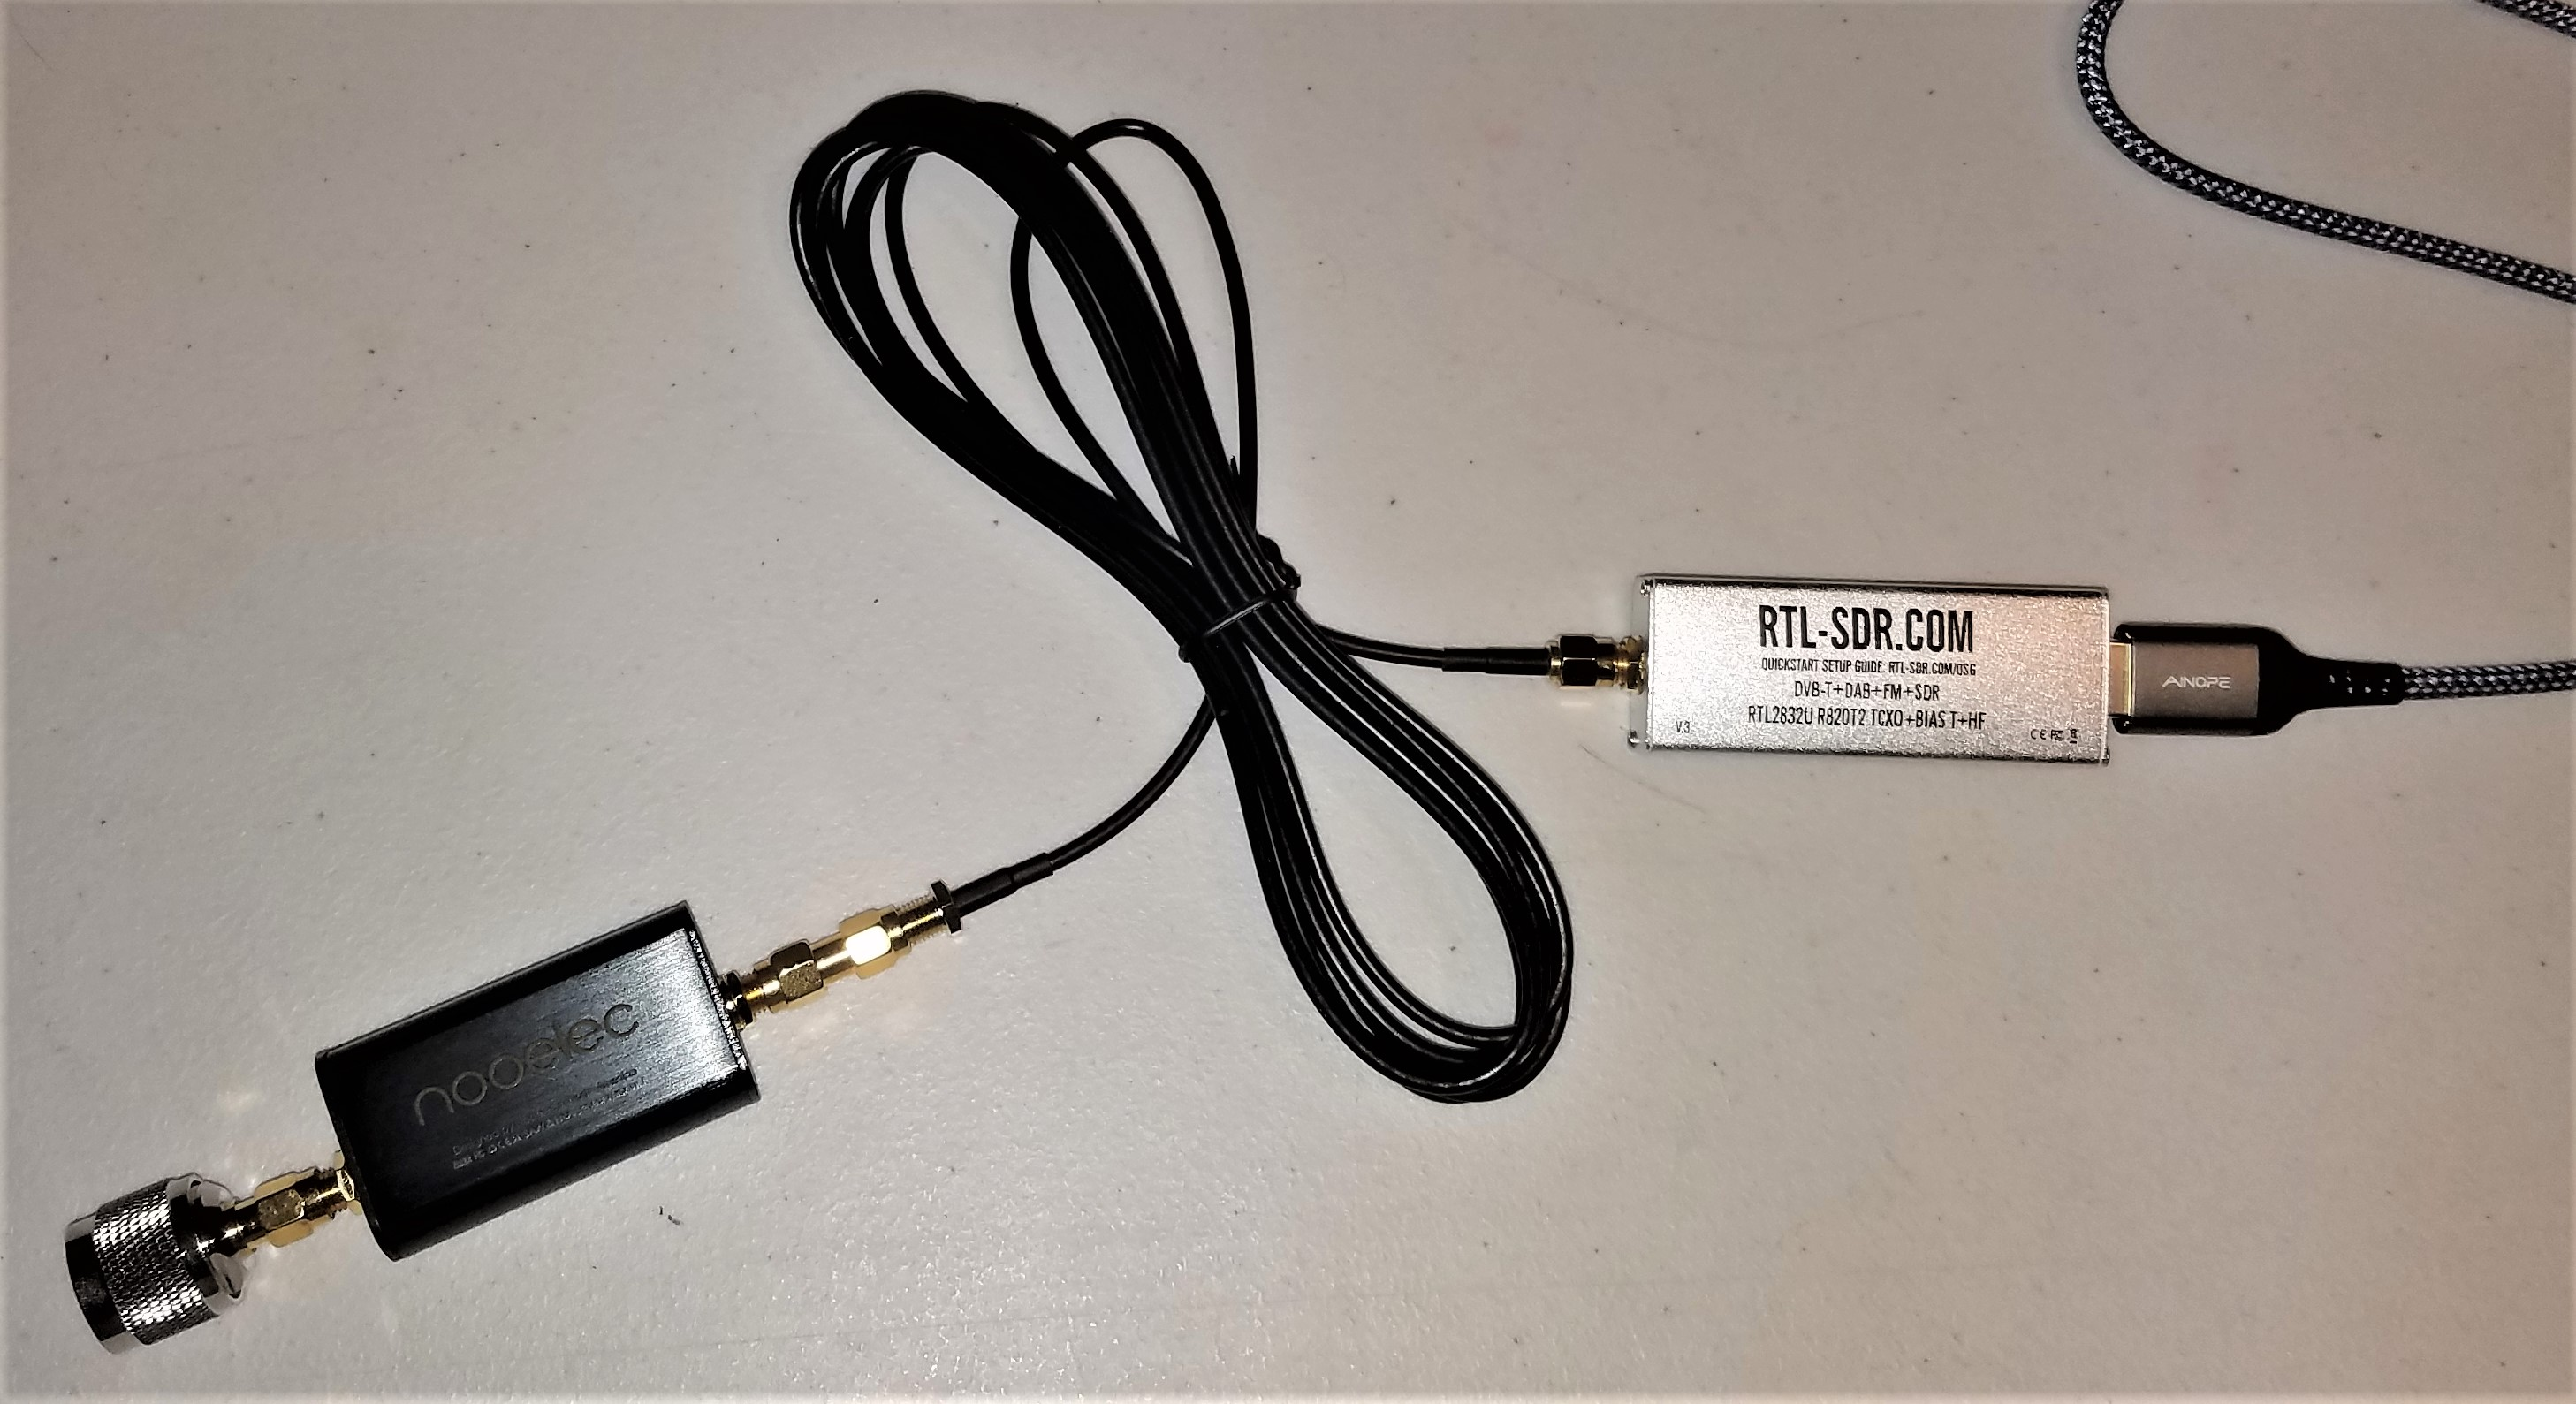
\includegraphics[width=0.75\textwidth]{RadioLabPhotos/adapter_to_lna_to_cable_to_sdr.jpg}
\end{figure}

\subsection{Take basic calibration data}
Disconnect the SDR dongle from the cable that connects it to the antenna.
Put the 50-ohm resistor on the end of the SDR dongle.

\begin{figure}[htp]
    \centering
    Attach the 50 ohm resistor to the SDR for the basic calibration steps. \\
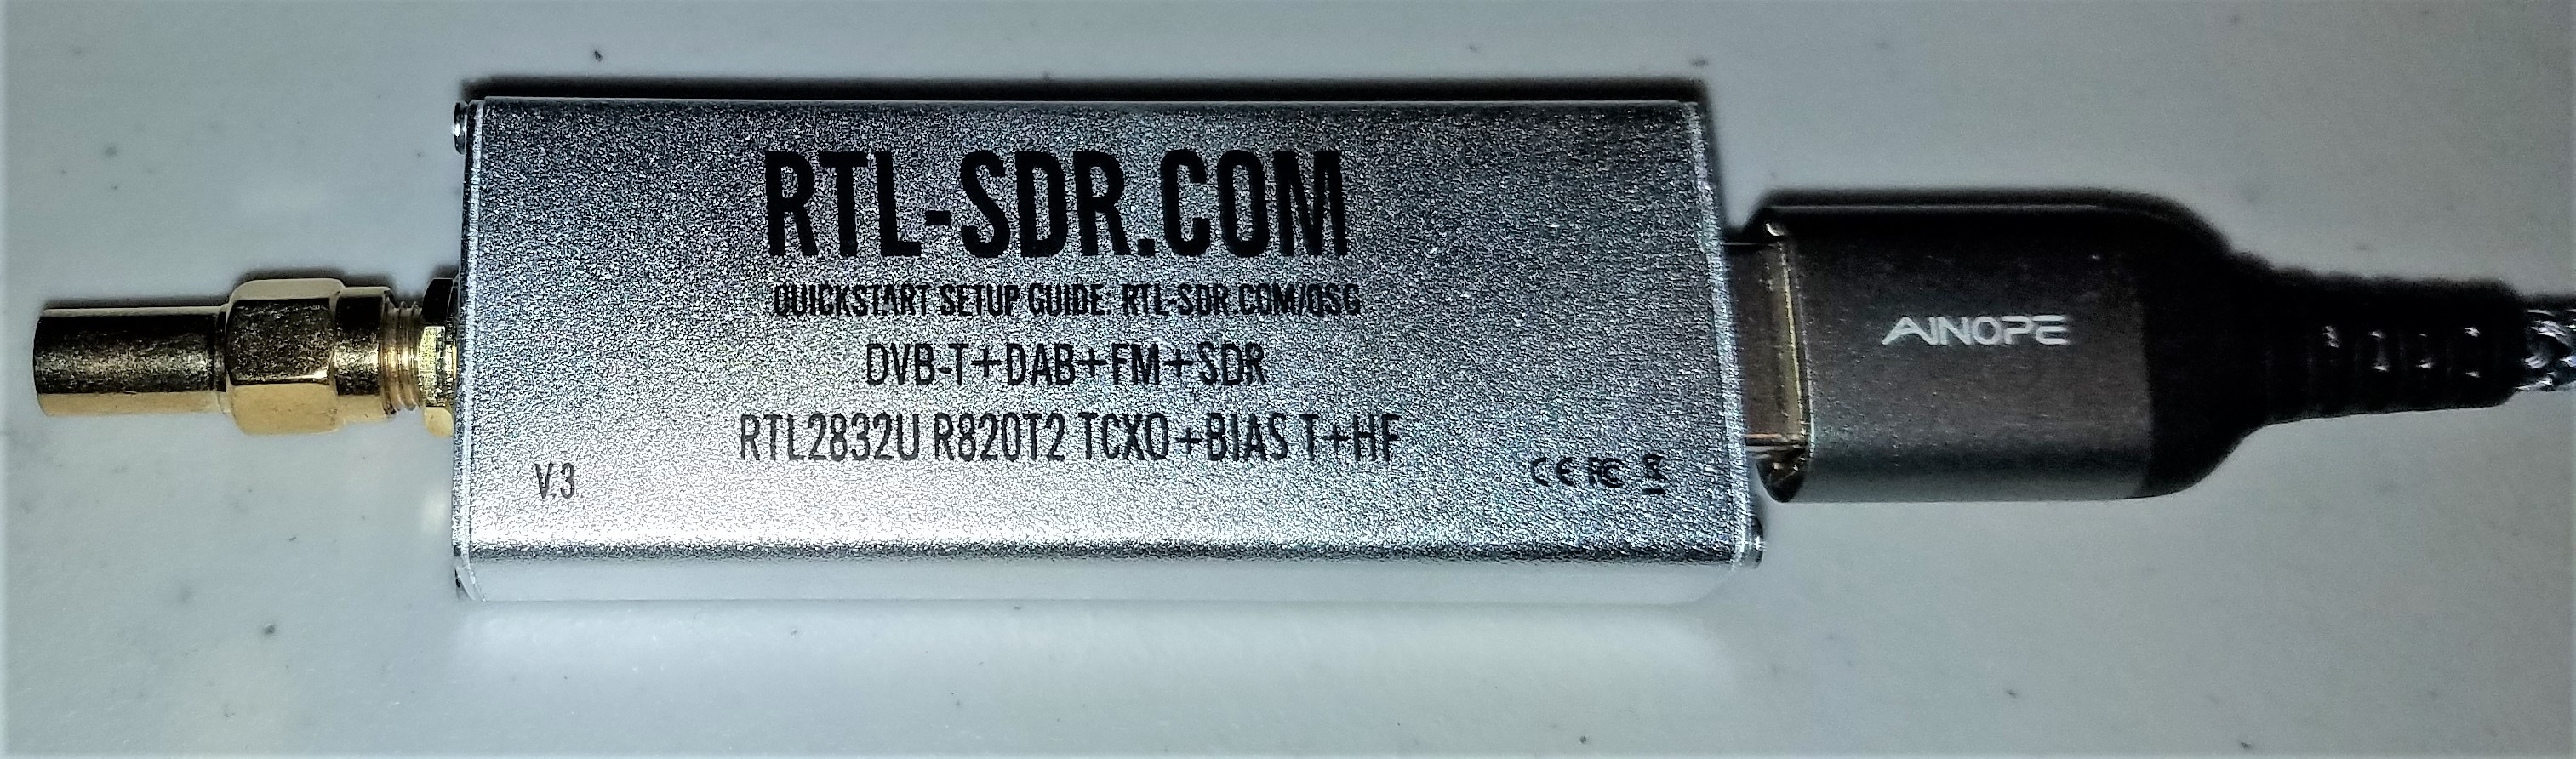
\includegraphics[width=0.75\textwidth]{RadioLabPhotos/sdr_with_resistor.jpg}
\end{figure}

Using the integration tool, take a 1-second and a 60-second integration.
You will do this using the \verb|run_sdrplay_integration| command.
Label these as \verb|50ohm_calibration| scans using the \verb|obs_type| keyword argument.
Take five (5) of each of the 1-second calibration scans by setting the sample time keyword \verb|sample_time_s=1|.  Take one (1) 60-second integration
for each configuration (resistor on, resistor off, LNA on with resistor, LNA on without resistor).
Set the filename appropriately for each configuration.
Set the altitude and azimuth both to -999 to indicate that this
is not a real on-sky observation.


Example \verb|run_sdrplay_integration| call:\\
\begin{verbatim}
run_sdrplay_integration(altitude=-999, azimuth=-999, sample_time_s=1,
                   observatory_longitude=-82.3, observatory_latitude=29.6,
                   obs_type='50ohm_calibration', freqcorr=0,
                   output_filename='50ohm_calibration_1s.rx')
\end{verbatim}

Recall that you can look at the documentation for a function with a \verb|?|, e.g.:
\verb|run_sdrplay_integration?|.  There are many other keyword arguments that may be needed;
see Section \ref{sec:troubleshooting} below.



\begin{figure}[htp]
    \centering
    The LNA should be connected to the coax cable via the male-to-male adapter\\
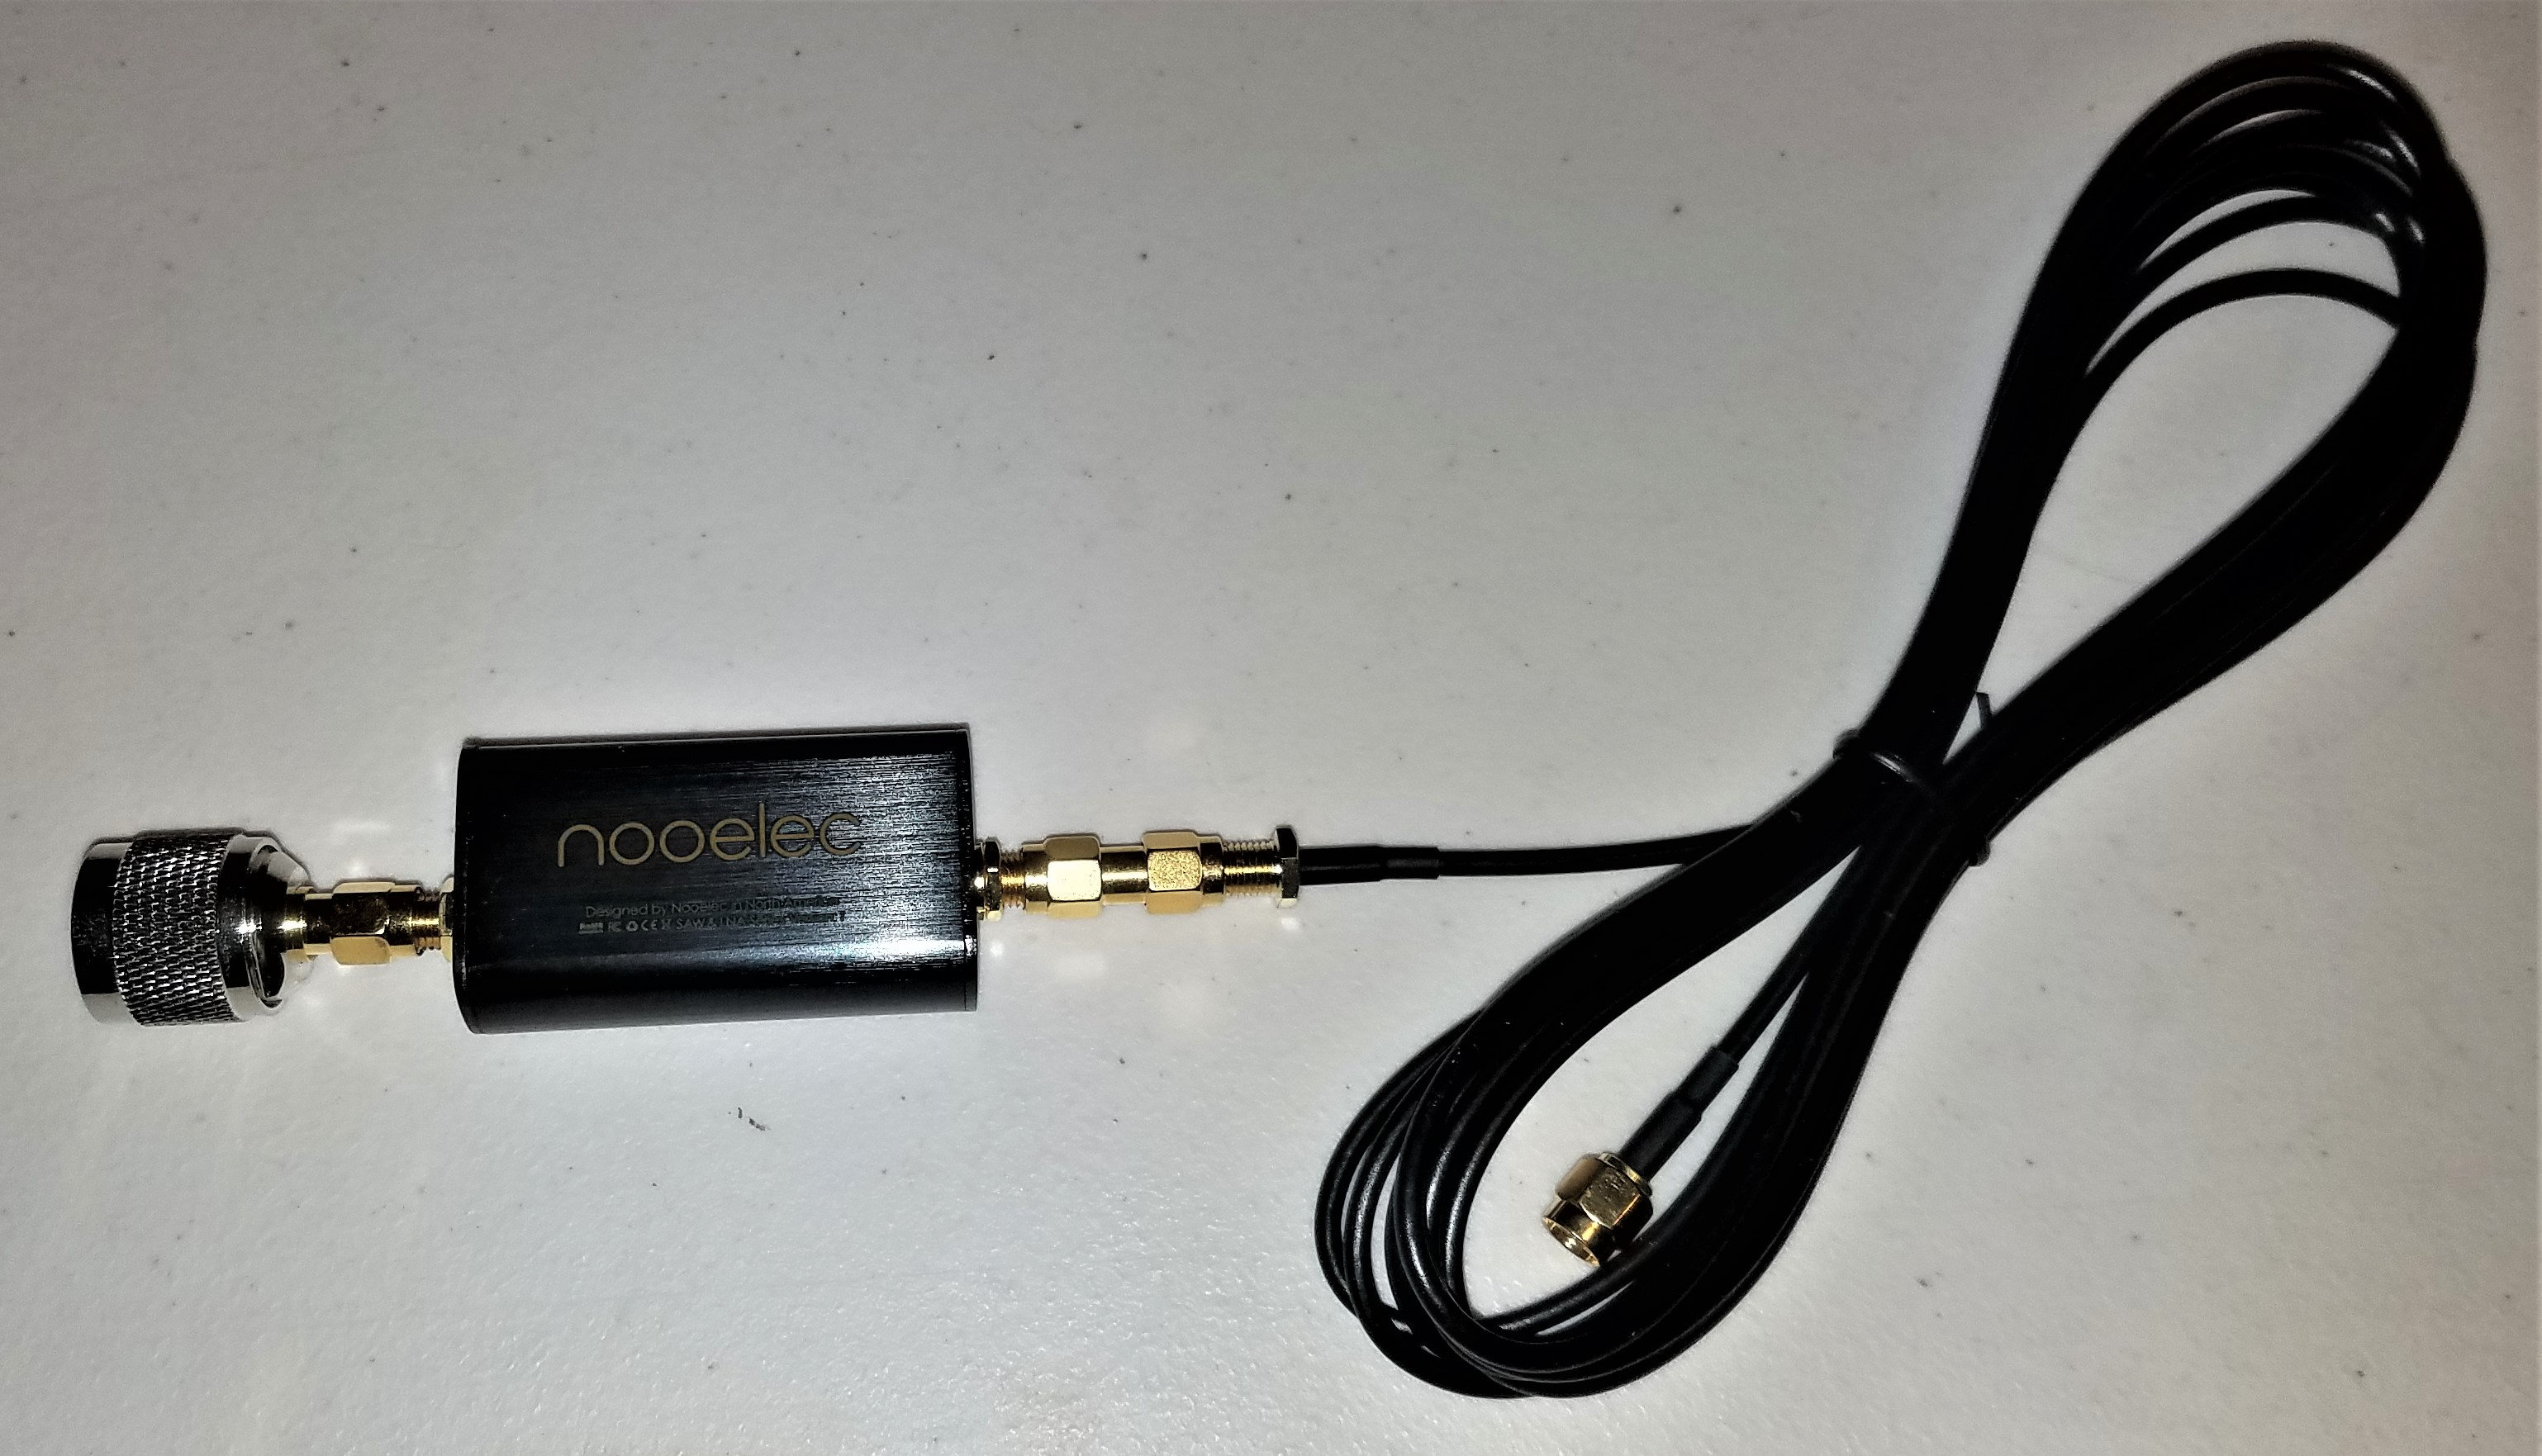
\includegraphics[width=0.75\textwidth]{RadioLabPhotos/coaxcable_to_LNA.jpg}
\end{figure}

\subsubsection{Frequency Calibration}
\label{sec:freqcal}
Now, attach the dipole antenna to the SDR.
Make sure the LNA is not in the signal path, i.e., not plugged in!  (the LNA includes filters that will block the NOAA signals we're going to use)
Use the \verb|run_sdrplay_integration| command to take a frequency calibration measurement.
Record the ``Measured Frequency Offset'' it reports.
Repeat this measurement 10 times.
Record each value, then report the mean and standard deviation.
This value, rounded to the nearest integer, will be your frequency correction; we expect it to be near zero.

\begin{figure}[htp]
    \centering
    The SDR should be connected to the bunny-ear dipole antennae for the frequency calibration step.\\
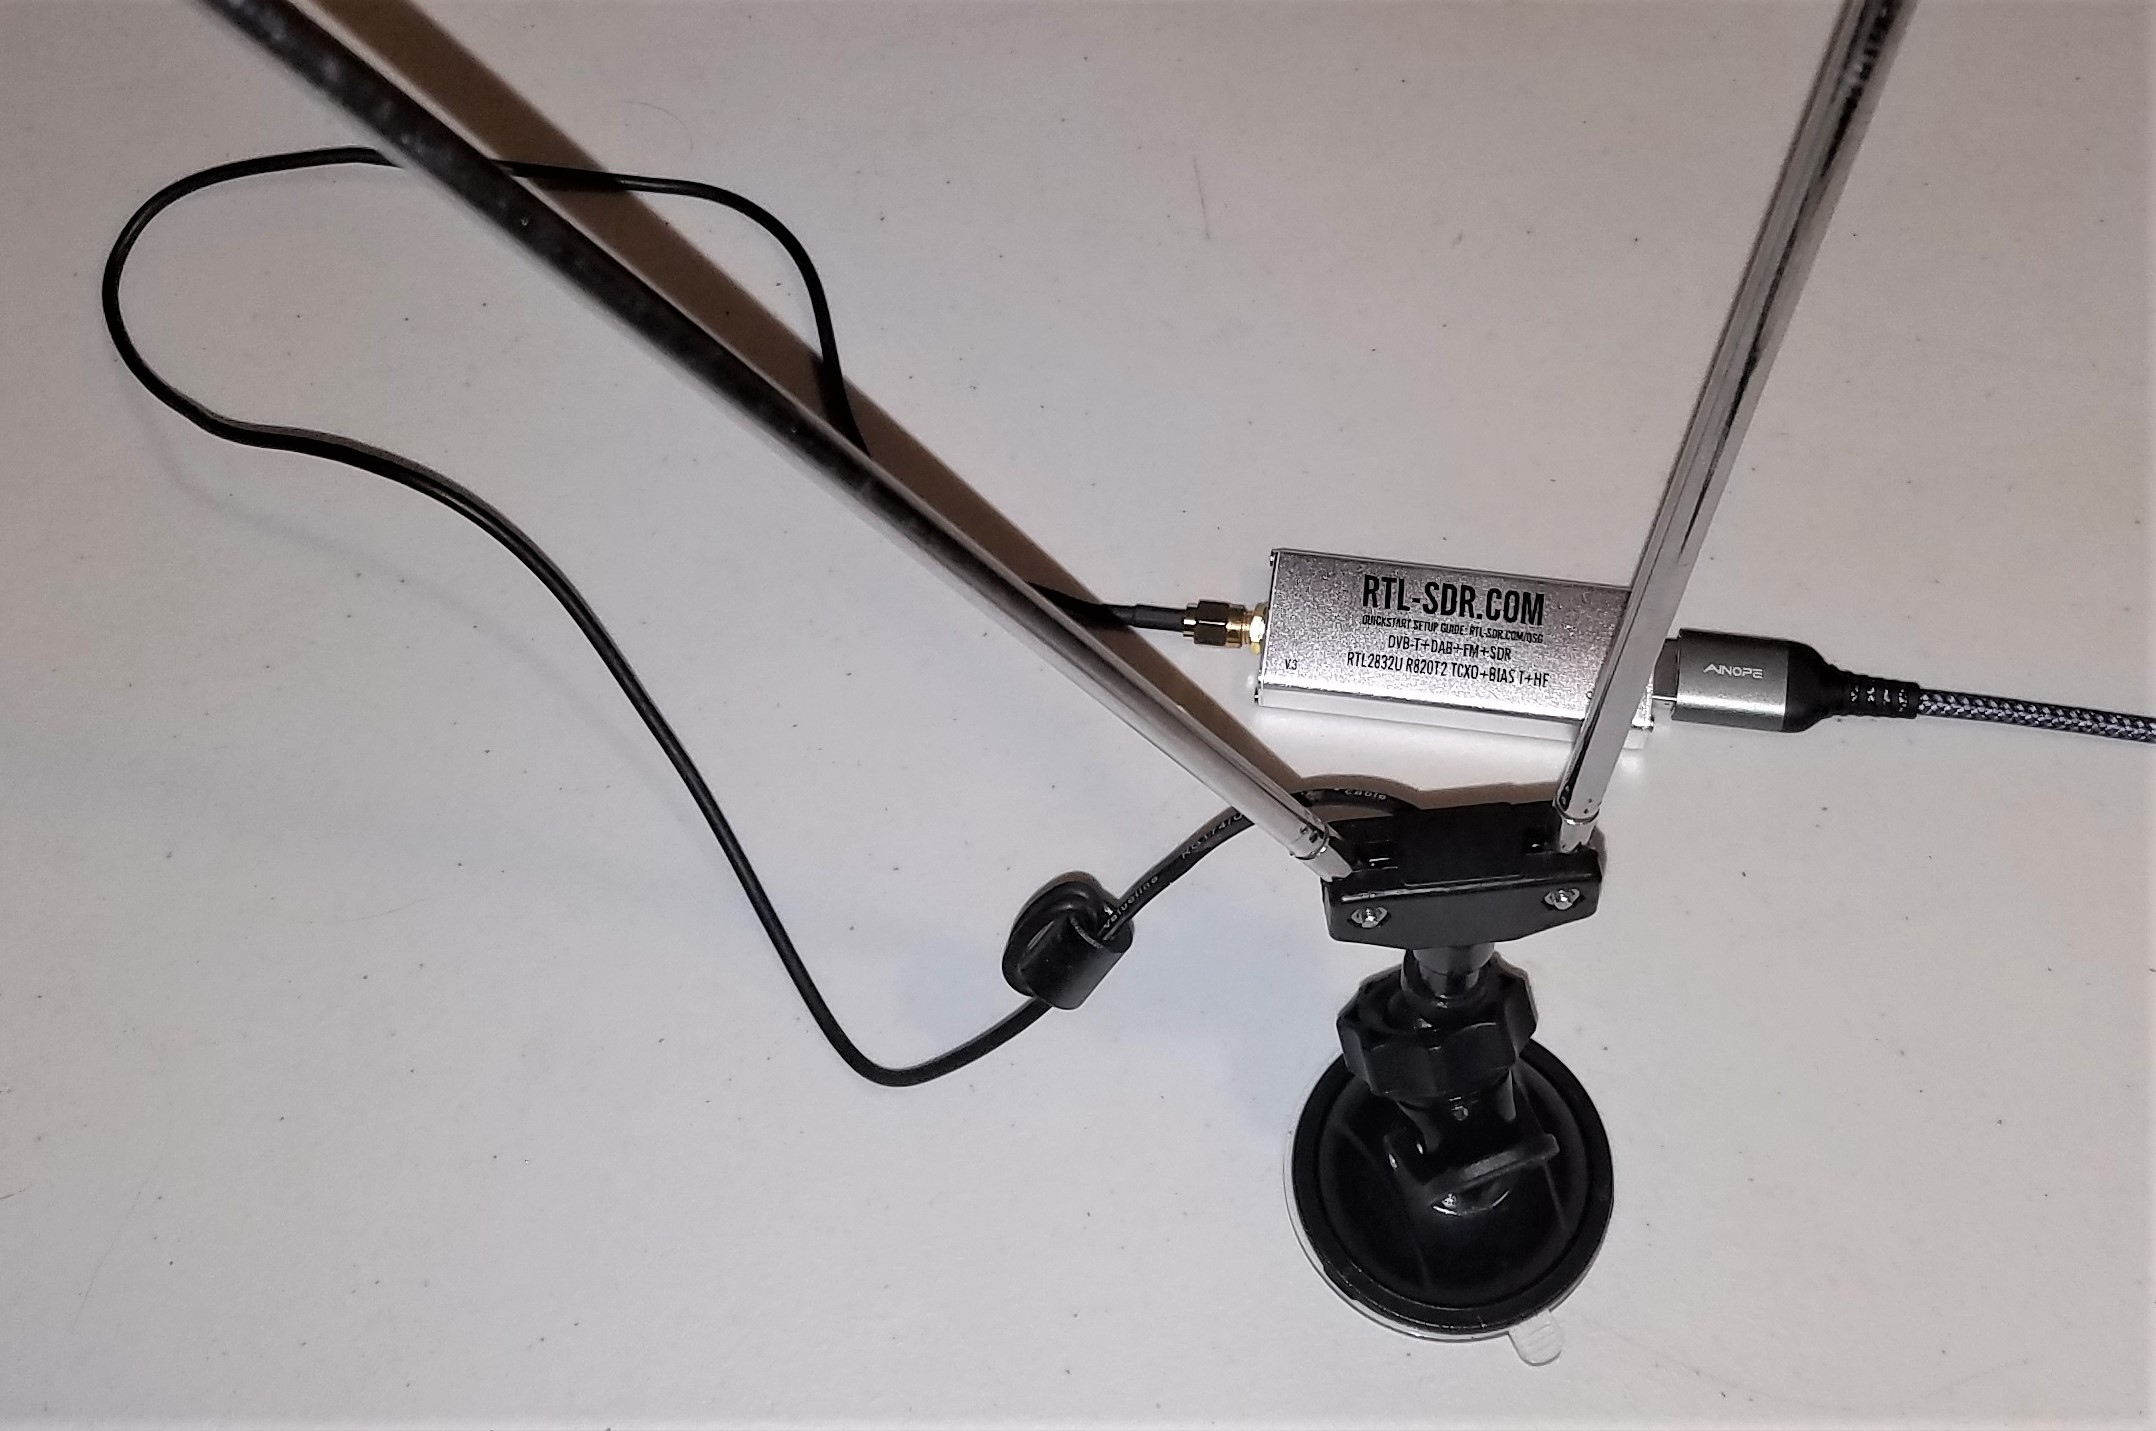
\includegraphics[width=0.75\textwidth]{RadioLabPhotos/sdr_to_bunnyears.jpg}
\end{figure}


\subsubsection{Plot the calibration data}
Now that you've taken some data, plot it!

Using \texttt{astropy.table}, read the files.
\verb|tbl = astropy.table.Table.read('filename_goes_here.fits')|

Plot the spectra.  There are a few different spectra to plot:
\begin{itemize}
    \item Plot column \verb|power1| on the y-axis against \verb|frequency1| on the x-axis
    \item Plot column \verb|power2| on the y-axis against \verb|frequency2| on the x-axis
    \item Repeat the above steps in different plot windows for each of the four
        calibration scans.  You should end up with a total of 8 plots, one pair for
        each of the calibration scan types.
    \item Label each plot by its integration time and whether it had the resistor
\end{itemize}

Question: (How) do the spectra differ?

\subsubsection{Frequency Switching}
\label{sec:fsw}
To obtain clean, calibrated data, we are using a techique called \emph{frequency switching},
in which we record data at two frequencies separated by more than the expected line-width,
but less than the receiver bandwidth.  In frequency switching, we integrate for two consecutive
observations, then take their difference.

Plot \verb|fsw_spectrum| vs \verb|frequency1| for each of the four spectra in a four-panel plot. \\
Use \verb|matplotlib.pyplot.subplot(2, 2, ii)| to make this four-panel plot.

Question: How do these spectra differ from the non-frequency-switched spectra?


\clearpage
\section{Observe your target}
\label{sec:observe}
\subsection{Set up the radio telescope antenna}
At your selected site, set up the antenna and observing station.

\begin{enumerate}
    \item Scout out the location, make sure it's clear
    \item Set up the tripod
    \item Put the mount in the tripod
    \item Attach the dish to the mount
    \item Point the dish toward the target altitude, then tighten the altitude-locking screws
    \item Measure how far the feed is off of zenith (i.e., measure the altitude).
    \item Set up your observing station (your computer and SDR)
    \item Connect the LNA to the antenna feed using the big-to-little adapter
        (the side with the micro-USB port should be pointed toward the antenna
        feed).  Double-check that you have this right, and take a photo of the connection to turn in with your report.
    \item Connect the coax cable to the LNA
    \item Connect the other end of the coax cable to the SDR via the little-to-little adapter
    \item Turn on the computer
    \item Plug the dongle into the USB extension cord
    \item Plug the USB extension cord into the computer
\end{enumerate}

For your writeup, be sure to note: Did you do anything differently from the above?
Were there any steps left out of these instructions (it's very possible something important
and obvious was left out!).


\begin{figure}[htp]
    \begin{minipage}{0.45\textwidth}
    \centering
        The LNA should connect to the antenna cable through the large adapter, attached on the side that has a micro-usb-in.\\
        \vspace{3mm}
    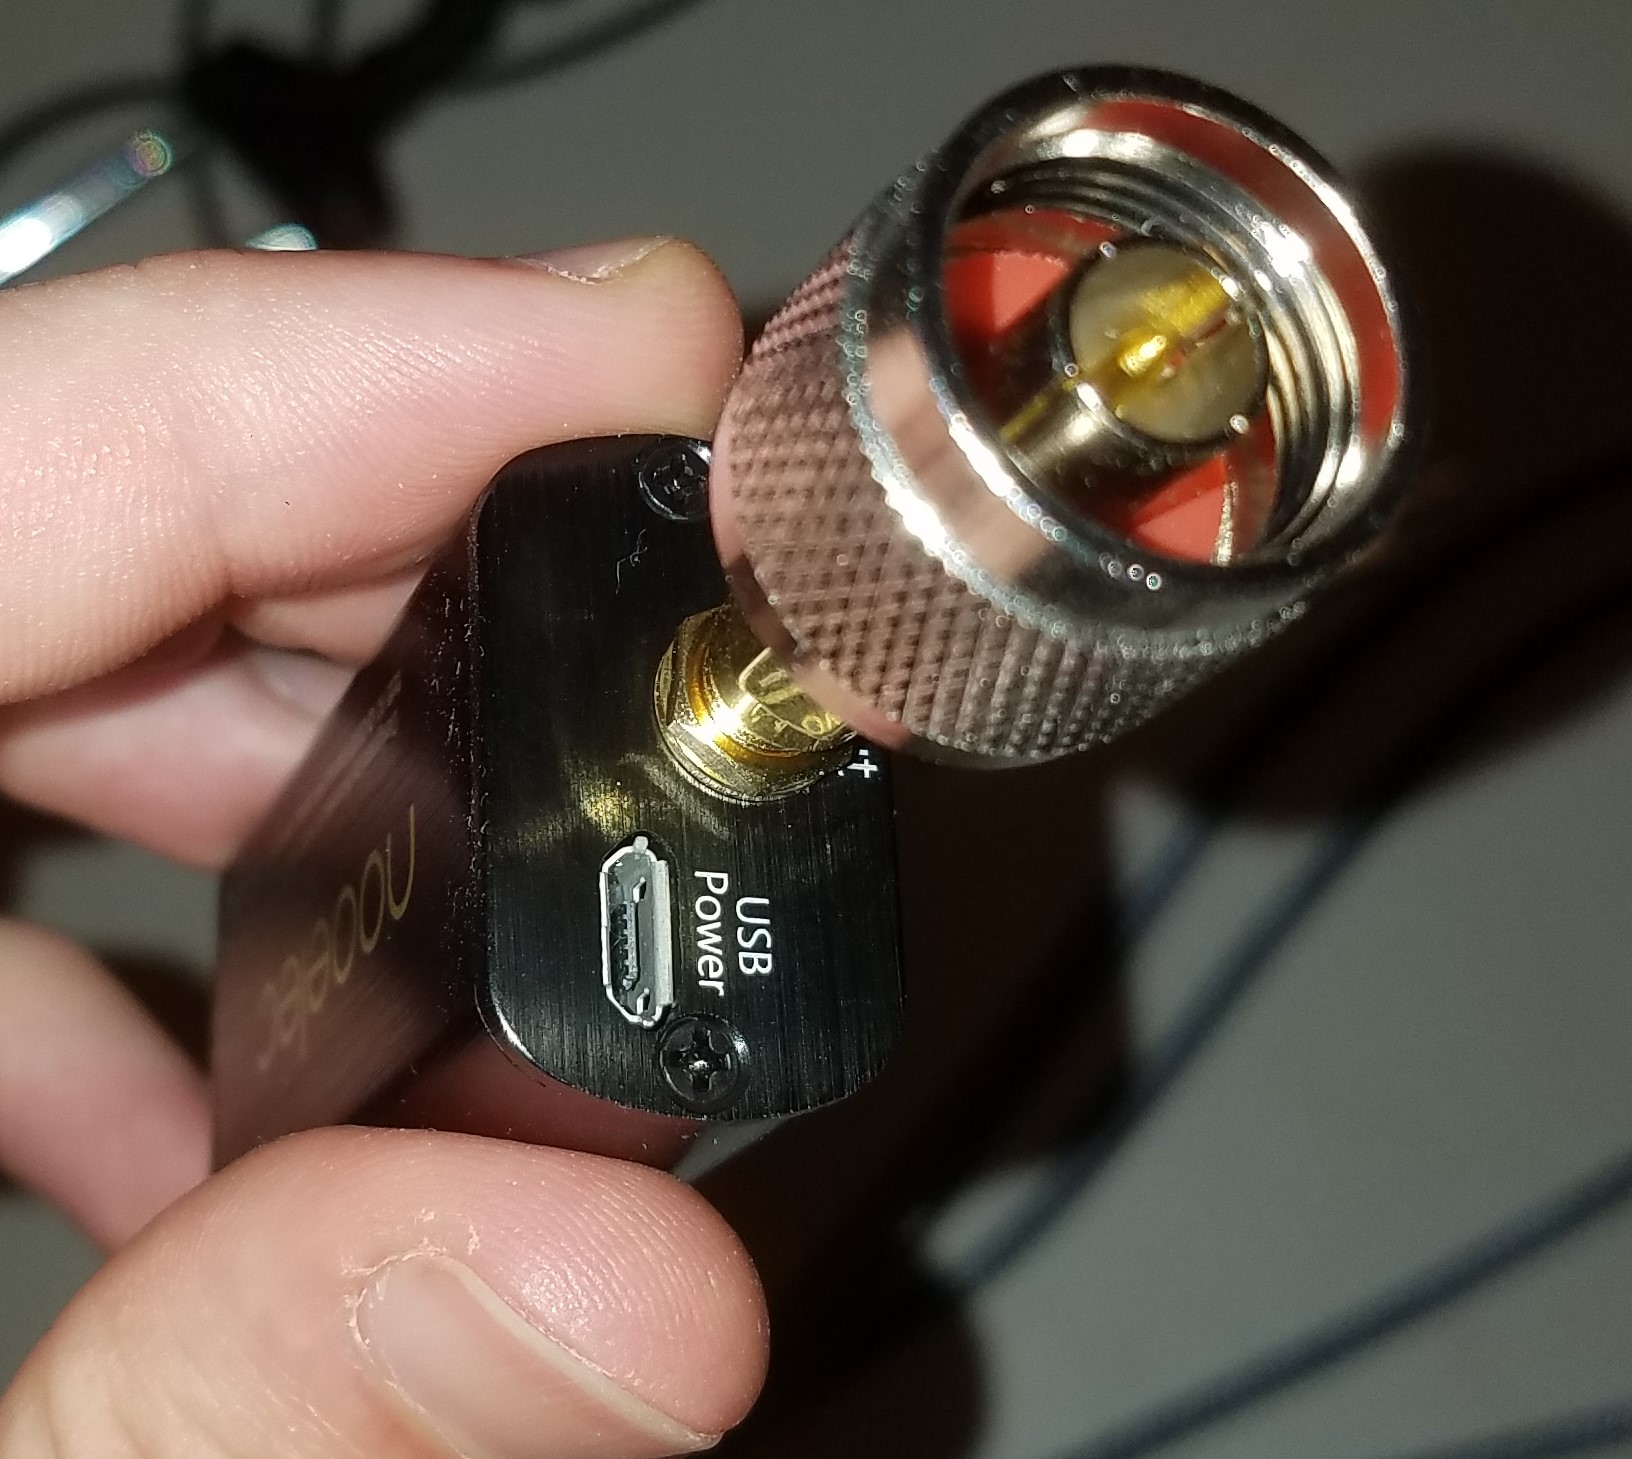
\includegraphics[width=0.65\textwidth]{RadioLabPhotos/coax_adapter_on_LNA.jpg}
    \end{minipage}
\end{figure}


\par Do the observations!

Make sure to keep an observing log for this session.  Use a spreadsheet, either google docs or excel.

\begin{tabular}{|c|c|c|c|c|c|c|c|}
\hline
Observation ID & Observation Time & Altitude & Azimuth &  Gal. Longitude & Gal. Latitude  & $t_{int}$ & Notes \\
\hline
 1  & & & & & & & \\
 \hline
 2  & & & & & & & \\
 \hline
\end{tabular}

\subsection{Point the telescope at the target}
\label{sec:point}
Using the adjustable screws, loosen the altitude mount until it can swing freely - \emph{be sure to hold on to it} so it doesn't fall over!
Adjust the antenna to point at the desired altitude.
Measure that you're pointing at this altitude using your tool (e.g., your phone app).
Record what you measured, and record the time you made the measurement.
Once it is pointed at the right altitude, lock in the screws to hold pointing fixed.

Rotate the telescope to point at the correct azimuth.
Use a compass; note that the magnetic declination (difference between magnetic
and true north) in Florida is about 5$^\circ$.
Remember that azimuth starts from 0$^\circ$ to the north, is $90^\circ$ to the east,
and is 180$^\circ$ to the south.
The telescope should easily stay pointed at the appropriate azimuth without
any locking mechanisms as long as you don't bump it.


\subsection{Obtain an integration}
\label{sec:integrate}
Before you start taking data, make sure your computer's clock is correct.


To record data, remember you need to pass several parameters to the \verb|run_sdrplay_integration| command:
\begin{itemize}
    \item \verb|altitude| and \verb|azimuth| must be set to the telescope's alt and az
    \item The observatory latitude and longitude must be set correctly
    \item \verb|obs_type| should be ``science''
    \item The integration time (\verb|sample_time_s|) should be set to 1 minute (60s).
    \item \verb|output_filename| should be set to a unique filename.
\end{itemize}

If you're doing a drift scan, see the Drift Scan section (\S \ref{sec:driftscan}) below.

Plot your data.  Take notes:
\begin{itemize}
    \item Did you detect the HI emission line?
    \item What is the approximate velocity of the HI emission line?
    \item Is there Radio Frequency Interference (RFI)?
\end{itemize}

\subsection{Observe all your targets}

(if you're doing a drift scan, you can skip this section and go to the Drift Scan section (\S \ref{sec:driftscan}) below)

Repeat the steps in \S \ref{sec:point} and \ref{sec:integrate} for each target you have selected.

By the end of this observing session, you should be able to create a data table like this:

\begin{tabular}{|c|c|c|c|}
\hline
 Observation ID &   Galactic Longitude & Galactic Latitude & Velocity Peak of HI \\
\hline
 1  & $\ell= ?? ^\circ$ & $b= ?? ^\circ$ & ?? km s$^{-1}$ \\
 \hline
 2  & ... & ... & ... \\
 \hline
 3  & ... & ... & ... \\
 \hline
\end{tabular}

\subsection{Observe the Sun}
In order to calibrate the antenna, we need to observe the sun.  During the day,
calculate a position the Sun will pass through.  Point the telescope at that
position starting \emph{at least} 1 hour before the sun passes through the
target position and keep recording for \emph{at least} 1 hour after.


Alternatively, you may take three measurements consecutively by pointing away
from the sun, at the sun, then away from the sun in one observing session.  If
you do this, make sure you carefully point at the sun during the on-sun
pointing.  It may be a good idea to continuously integrate (i.e., constantly
take observations) while you are pointing toward and away from the sun, and
simply note the timestamps (filenames) of the data from when you successfully
took data vs those where you did not.  See the Drift Scan section (\S
\ref{sec:driftscan}) below for instructions on how to do this.

\subsection{Drift Scan}
\label{sec:driftscan}

For drift scans, you will continuously obtain integrations.
This can be done by running the \verb|run_sdrplay_integration| command in a loop.

\begin{verbatim}
    while True:
        now = str(datetime.datetime.now().strftime("%y%m%d_%H%M%S"))
        run_sdrplay_integration(altitude=altitude, azimuth=azimuth, sample_time_s=60,
                                obs_type='science', output_filename=f'HI_drift_alt{altitude}_az{azimuth}_60s_{now}.rx')
\end{verbatim}

The \texttt{now} variable contains a unique timestamp for each file.

If you use this approach when observing the sun, change the label from \texttt{HI\_drift} to \texttt{Sun\_drift}.



\subsection{Data Packaging and Delivery}
Once you've acquired data for all of your targets and the corresponding calibration data, you're done observing.

You will need to upload all of the data \emph{and} your observing log.
Your log should be in spreadsheet form.  If you used
google sheets, export the file to excel format on the observing computer.

Create a \texttt{README} file describing the data.  Open a text file,
and put in the file:
\begin{enumerate}
    \item your name
    \item the date
    \item the number of files
    \item the total size of files
    \item any notes about mis-labeled files or things that might have gone wrong
    \item the name of the observing log file
\end{enumerate}

Then, zip up the files, including the README, the log, the FITS files, and any plots
and notebooks you want to save:
select all of the files you want to upload in Windows Explorer, right click on
them, and select ``Send to'' $\rightarrow$ ``Compressed (zipped) Folder''.

Upload the zip file to canvas.
%If we run out of space on canvas, we might have
%to switch to dropbox or onedrive, but we'll start with canvas.


\section{Analysis}

From your solar observation, determine what the `gain' factor is.  This is your primary
calibration term for converting your measurements from arbitrary amplitude into meaningful
intensity measurements.


For each of your spectra, determine:
\begin{enumerate}
    \item Did you detect an HI signal?
    \item What was the observed centroid velocity of that signal?  Its width?  Its amplitude?
    \item What is the uncertainty on those measurements?
    \item What was the velocity of your observatory in the direction of the signal
        at the time of observation?
    \item What is the observed velocity in the local standard of rest?
\end{enumerate}

You will aim to make a map of your data in Galactic coordinates.
Using the tools shown in the ``Observation Planning into Map Making" lecture
(https://ufl.instructure.com/courses/462047/assignments/5416346),
create a cube of the data.
Then, produce a ``moment-0'' map by taking the sum of the cube along the spectral
axis.

Combining the data cube with the information from the ``Velocity and Galactic
Rotation'' lecture, can you infer the mass of the Milky Way?


\section{Writeup}

Copied from above, this is the breakdown of the lab writeup:
\begin{enumerate}
    \item Introduction (5\%): Describe the purpose of the lab \& background
    \item Procedure (55\%): Describe the setup of the hardware and the data taking process
    \item Data Analysis (25\%):  Report and analyze your measurements
    \item Data Packaging and Delivery (10\%): Put the data together and turn them in with appropriate metadata
    \item Conclusions (5\%): Summarize what you learned
\end{enumerate}


The Procedure section should include your observing log.

The Data Analysis section should include plots of the data.
You will likely need to download the zip file you uploaded to canvas
so you can include appropriate plots.






\section{Troubleshooting}
\label{sec:troubleshooting}
\subsection{The LNA light doesn't turn on}

Is it plugged in?\\

Is it pointing the right way?  (micro-usb side should face toward the feed, away from the SDR)\\

Is the SDR plugged in to the USB port?\\
Try the other USB port(s) on the computer.  Does it work now?\\


\subsection{I get an error when I run \texttt{run\_sdrplay\_integration}}
There are many possible errors.

If there is an error but you can't figure out what it is,
try setting \verb|verbose=True| to see if you can get some
debugging information, and share that with the instructor \& TA.




\subsection{The device isn't recognized}

If you get an error like this:
\begin{verbatim}
RuntimeError: SoapySDR::Device::make() no match
\end{verbatim}
it means the computer was unable to recognize the SDR.

\begin{itemize}
    \item Make sure the SDR is plugged in to the USB port.
    \item Make sure no other software is using the SDR (e.g., SDRConnect)
    \item Unplug and replug it
\end{itemize}

You can verify that the SDR can be found by running this command:

\begin{verbatim}
    import SoapySDR
    print(dict(SoapySDR.Device.enumerate()[0]))
\end{verbatim}

which should print
\begin{verbatim}
    {'driver': 'sdrplay',
     'label': SDRplay Dev0 RSPdx-R2 .......',
     'serial': '........'}
\end{verbatim}

You can also run the command-line commands:
\begin{verbatim}
    SoapySDRUtil --find
    SoapySDRUtil --probe="driver=sdrplay"
\end{verbatim}



\section{Appendix: Reading and Plotting}

You should be able to read the data using the \verb|astropy.table| package.

\begin{verbatim}
    from astropy.table import Table
    tbl = Table.read('filename_goes_here.fits')
\end{verbatim}

You can plot the data using \verb|matplotlib.pyplot|.

\begin{verbatim}
    import matplotlib.pyplot as plt
    plt.plot(tbl['frequency'], tbl['power'])
    plt.show()
\end{verbatim}

There are also tools built in to the \verb|run_sdrplay_integration| script to plot the data:

\begin{verbatim}
    plot_table('filename_goes_here.fits')
\end{verbatim}

If you take many spectra in a row, e.g., for a drift scan, you can make waterfall plots.
These are plots with frequency on the x-axis and time on the y-axis with every pixel filled and colored by the brightness of the spectrum.

The raw data files, \verb|*.rx|, are numpy arrays that can also be plotted if \verb|cleanup=False| is passed to \verb|run_sdrplay_integration|.
You don't generally want that, because these files can be huge.
However, if you want to look at one example, which can be useful to look for radio frequency interference (RFI), you can make a waterfall plot of these data too:

\begin{verbatim}
    waterfall_plot('filename_goes_here.rx')
\end{verbatim}




\end{document}
% resource: https://www.youtube.com/watch?v=_eMNRa-KEiQ
